\section{802.11ah and \gls{raw} \label{subsec:802.11ah} }
%\begin{itemize}
%\item Explanation of 802.11ah: RAW, min and max MCS, adaptive rate control


 
Like the legacy 802.11ah technologies, in physical layer, 802.11ah supports multiple transmission rate represented by \gls{mcs}. As listed in table \ref{tab:wifi-modes},  the number of supported MCS depends on the channel width, for channel width 1 MHz,  MCS 0 $\sim$ MCS 10 are supported with transmission data rate ranging from 150 Kbps to 4 Mbps, and for 2 Mhz, MCS 0 $\sim$ MCS 9 are supported with transmission data rate ranging from 650 Kbps to 7.8 Mbps, more details can be found in \cite{802.11ahStandard}. The stations are allowed to dynamically choose the MCS  for packet transmission to adapt to the conditions of the wireless channel.

% Table I lists data rates and their MCSs
% when GI and NSS are 8 us and 1, respectively for 1 and 2 MHz
% bandwidth.


\begin{table}[t]
\centering
\caption{802.11ah MCSs for 1, 2~MHz, NSS=1, GI=$8~\mu{}s$}
\label{tab:wifi-modes}
\begin{tabular}{ccccc}
\hline
\multirow{2}{*}{\begin{tabular}[c]{@{}c@{}}MCS\\ Index\end{tabular}} & \multirow{2}{*}{Modulation} & \multirow{2}{*}{\begin{tabular}[c]{@{}c@{}}Coding \\ rate\end{tabular}} & \multicolumn{2}{l}{Data rate (Kbps)} \\ \cline{4-5} 
 &  &  & 1 Mhz & 2 Mhz \\ \hline
0 & BPSK & 1/2 & 300 & 650 \\ 
1 & QPSK & 1/2 & 600 & 1300 \\ 
2 & QPSK & 3/4 & 900 & 1950 \\ 
3 & 16-QAM & 1/2 & 1200 & 2600 \\ 
4 & 16-QAM & 3/4 & 1800 & 3900 \\ 
5 & 64-QAM & 2/3 & 2400 & 5200 \\ 
6 & 64-QAM & 3/4 & 2700 & 5850 \\ 
7 & 64-QAM & 5/6 & 3000 & 6500 \\ 
8 & 256-QAM & 3/4 & 3600 & 7800 \\ 
9 & 256-QAM & 5/6 & 4000 & Not valid \\ 
\multirow{2}{*}{10} & \multirow{2}{*}{BPSK} & 1/2 with 2x & \multirow{2}{*}{150} & \multirow{2}{*}{Not valid} \\
 & & repetition & & \\ \hline
\end{tabular}
\end{table}


As the 802.11 standards do not specify the way of adapting transmission rate, some rate control algorithms have been proposed and used on the real devices to select the appropriate MCS for packet transmission to adapt to the network condition during the past years, for example, Arf \cite{arf1997},  Aarf \cite{aarf2004}, Onoe \cite{Onoe} and Minstrel \cite{minstrel}. The main ideal of these algorithms is to adjust the transmission rate based on the frequency of successful and failed transmission accumulated in the past. 


\begin{figure}[t]
  \centering
   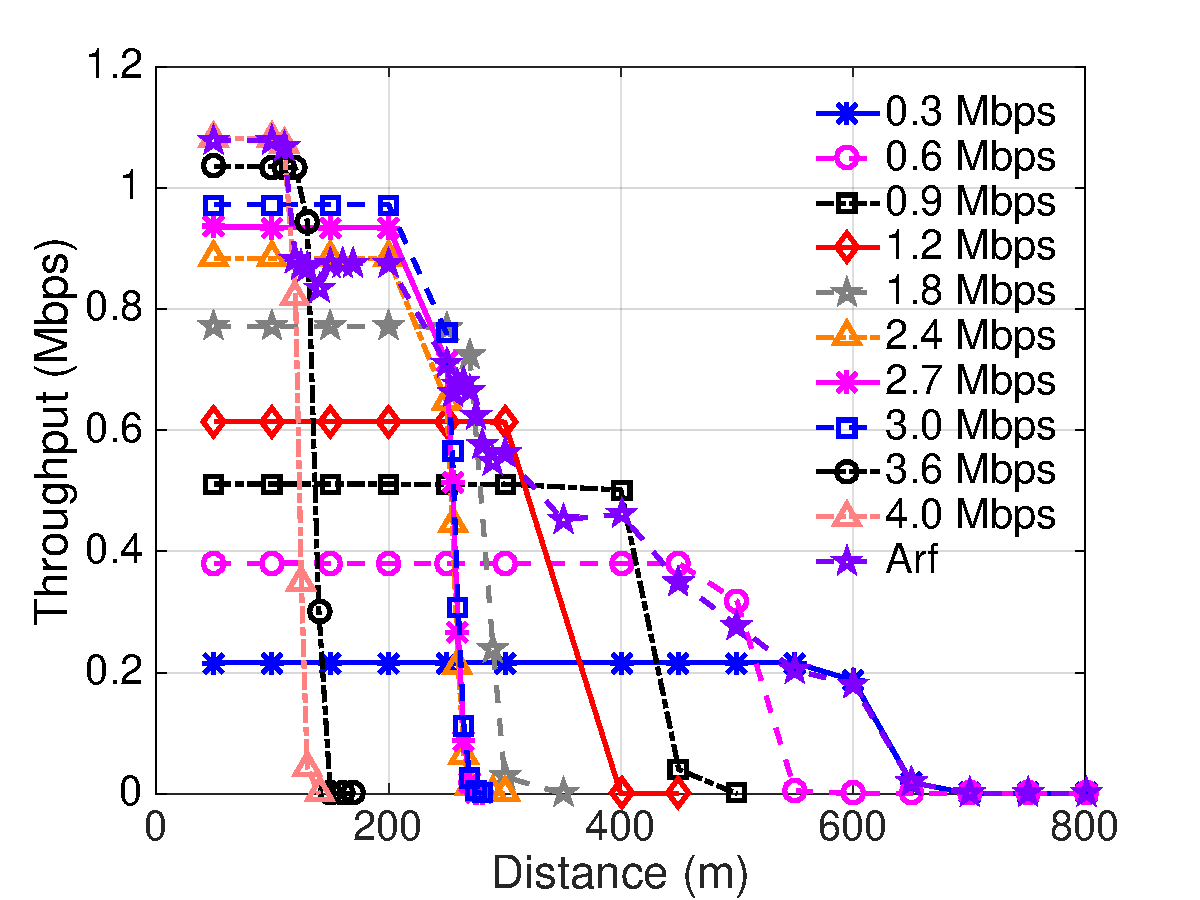
\includegraphics[width=0.45\textwidth]{figures/distance-throughput-512bytes}  \caption{The achievable throughput of each transmission data rate as a function of distance. \label{fig:dist-throughput}}
\end{figure}

\begin{figure}[t]
  \centering
   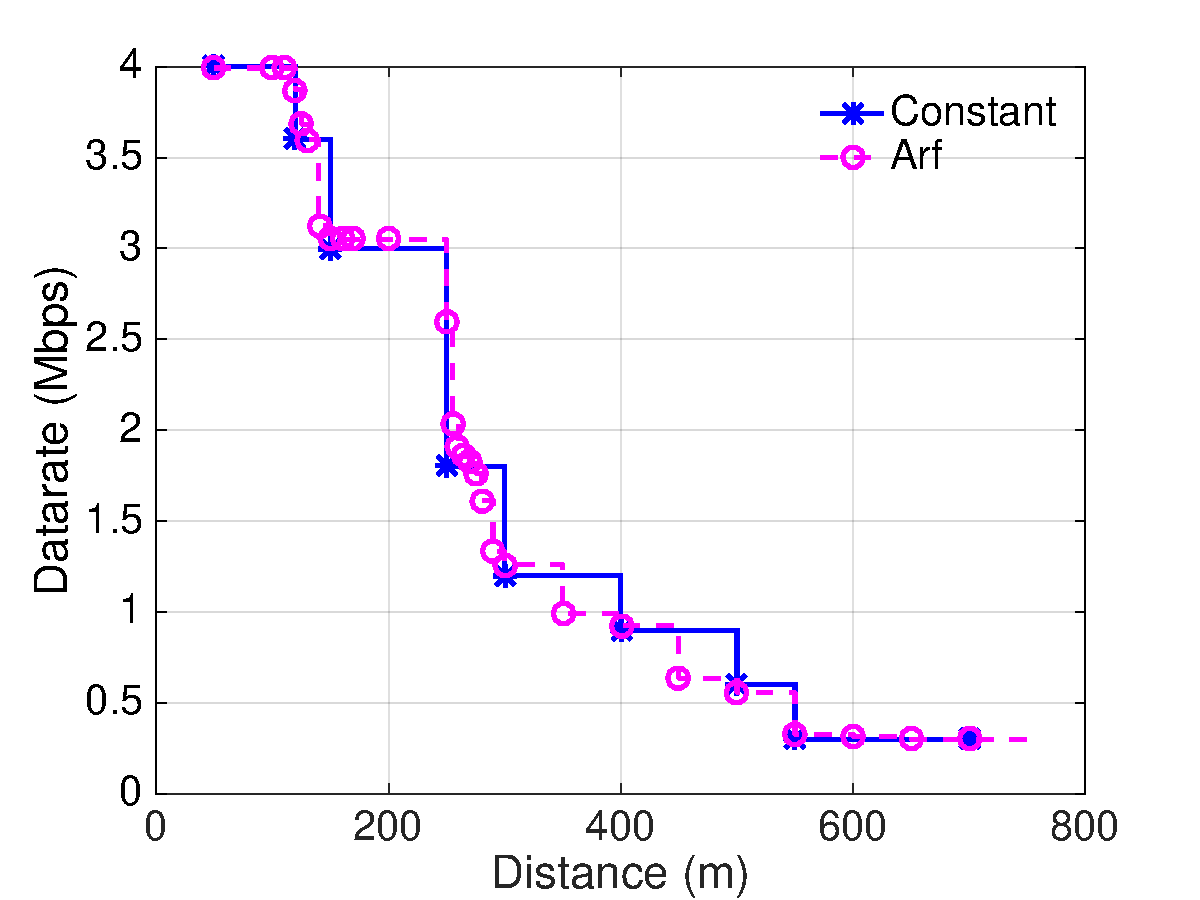
\includegraphics[width=0.45\textwidth]{figures/distance-datarate-512bytes}  \caption{The used transmission data rate for different distance distance. \label{fig:dist-datarate}}
\end{figure}

\textcolor{red}{Explain why not use current rca algorithm for modeling}. For the modeling, we use a simpler rate control method, allowing the stations to select the MCS solely based on its distance to the \gls{ap}, i.e., choosing the MCS which can stably achieve the maximal throughput at a certain distance. Figure \ref{fig:dist-throughput} shows the throughput when a station keeps sending packets (512 bytes) to the \gls{ap} at different distance using a certain transmission data rate, and with Arf algorithm as well. Based on the results, figure \ref{fig:dist-datarate} illustrates the rate control method used in the modeling, showing the selected transmission date rate for a certain distance.
% and the average data rate for a certain distance using arf.
Although the throughput is achieved with packet size 512 bytes, the same results can be achieved by other packet size as well (not depicted).


%Rbar \cite{rbar2001},

% frequency of successful failed transmission accumulated during
% a fixed invocation period of 1000 ms.

% In ARF, each sender attempts to use a higher transmission rate after a fixed number of successful transmissions at a given rate and switches back to a lower rate after 1 or 2 consecutive failures. Aarf is an improved version of Arf, we have chosen to adapt this threshold by using a binary exponential backoff When the transmission of the probing packet fails. Onoe is a credit based ragte control algorithm where the value of the credit is determined by the frequency of successful, erroneous and retransmissions accumulated during
% a fixed invocation period of 1000 ms.

% Minstrel is based solely on acknowledgement feedback. Consequently, estimates of future success probabilities6 at a given rate
% are based only on past success ratios at that rate. With a moderate frequency, frames are selected
% to probe presently unused rates, and feedback from
% those probe frames maintains the probability estimates
% for unused rates so that, should the current best rate
% deteriorate, there is some basis for immediately selecting
% a more successful rate (Section 5.2)8.

% In ns-3, multiple rate control algorithms are available, such as for example \textit{ArfWifiManager}, \textit{ConstantRateWifiManager} and \textit{MinstrelWifiManager}. In the original simulator, the IEEE~802.11ah device could only use these algorithms to adapt the \gls{mcs} within the same channel bandwidth. As IEEE~802.11ah supports multiple channel bandwidths (i.e., 1,2,4,8, and 16~MHz), we modified the \textit{WifiRemoteStationManager} class (the parent class of all the rate control algorithms) to allow automatic switching among different channel bandwidths.

%\item Training methodology (the evaluation scenario used for training)

